\documentclass[a4paper,10pt]{article}
\usepackage{src/preamble}

\begin{document}

\noindent
\begin{center}
	\textbf{{\Large MAGNETI SUPERCONDUTTORI}} \\
\end{center}

\noindent
\textbf{Autore: Alessandro Biagiotti} \textit{Università degli studi di Milano, Milano, Italia}
\\

\noindent
\textbf{INTRODUZIONE:}
\\
Come già introdotto nel documento dedicato alla parte teorica, in questo secondo documento mi
dedicherò a una trattazione più pratica delle tecnologie superconduttive che sono oggi più in
utilizzo nel campo della fisica delle alte energie, e non solo (basti pensare ad applicazioni
ingegneristiche per treni ad alta velocità \cite{maglev}).

I superconduttori sono materiali caratterizzati da un brusco annullamento della resistività ($R = 0$
e non $R \approx 0$) una volta raggiunta una certa temperatura, nota come temperatura critica.
\begin{figure}[h!]
	\centering
	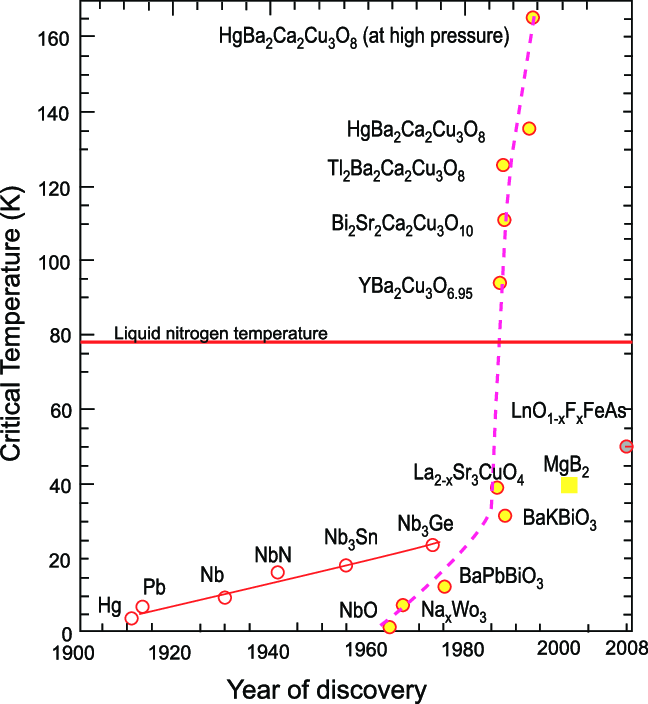
\includegraphics[scale=0.35]{fig/The-evolution-of-critical-temperatures-since-the-discovery-of-superconductivity.png}
	\caption{Temperatura critica di varie leghe che sono state scoperte nel corso degli
	anni \cite{critical-temp}}
\end{figure}
Il comportamento dei superconduttori puri è stato spiegato tramite la teoria BCS, risalente al 1957,
l'azzeramento della resistività del materiale è dovuto alla formazione delle cosiddette coppie di
Cooper.

Una coppia di Cooper è una coppia di elettroni che viaggiano insieme ed è generata da un'interazione
tra un elettrone e il reticolo cristallino (che è carico positivamente). Quest'interazione porta a
uno sbilanciamento della carica locale che passa da negativa a positiva pertanto pertanto è
possibile che un altro elettrone venga attratto, dando vita a una coppia di Cooper \cite{cooper-cambridge}. Una spiegazione più dettagliata del fenomeno mette in relazione questo comportamento con uno scambio di fononi \cite{quantum-springer}.

In un normale conduttore la resistenza elettrica sarebbe generata dallo scattering degli elettroni dovuto a collisioni con i nuclei positivi del reticolo cristallino. All'interno di un superconduttore, però, la maggioranza degli elettroni sono coppie di Cooper. Queste coppie, sebbene
interagiscano con il reticolo cristallino, non ricevono abbastanza energia per spezzare il legame che le tiene insieme e, di fatto, non si dividono negli elettroni che le formano; pertanto non vanno
incontro allo scattering che caratterizza la normale resistenza elettrica dei conduttori \cite{bcs-cambridge}. Questa mancanza di resistenza ovviamente consente di spingere al limite la quantità di corrente e la tensione che si possono applicare ad un superconduttore (dato che la resistenza è $0$ questo non può bruciare, fintanto che rimane in condizioni di criogenia).

All'interno di questo documento andrò ad esporre quali siano le tipologie di superconduttori attualmente in esistenza e infine esplorerò alcune delle leghe più utilizzate e alcune tecnologie più innovative nel campo della superconduzione a temperature elevate.

\bigskip
\phantomsection
\makeatletter\def\@currentlabel{\texttt{(II)}}\makeatother
\label{sec:quench}
\noindent
\textbf{SUPERCONDUTTORI DI TIPO I:}

\bigskip
\phantomsection
\makeatletter\def\@currentlabel{\texttt{(III)}}\makeatother
\label{sec:mariotto}
\noindent
\textbf{SUPERCONDUTTORI DI TIPO II:}

\bigskip
\phantomsection
\makeatletter\def\@currentlabel{\texttt{(III)}}\makeatother
\label{sec:mariotto}
\noindent
\textbf{CENNI DI METALLURGIA:}

\bibliography{tech}

\clearpage

\end{document}
